\documentclass{report}  
\usepackage[utopia]{mathdesign} 
%\usepackage{amsmath,amsfonts,amsthm,amssymb,mathtools}

\usepackage[french]{babel} 
\usepackage[utopia]{mathdesign}

% Pour emojis et autres symbols de Extansive LaTeX symbols list 

% Permet d'ajuster la taille des marges et de la distance pour les footer
\usepackage[tmargin=2cm,rmargin=0.4in,lmargin=0.4in,bmargin=2cm,footskip=.2in]{geometry}

% Permet d'optimiser l'affichage de différents symboles et formules mathématiques
\usepackage{amsmath,amsthm,mathtools}
\usepackage[clock]{ifsym}
\usepackage{karnaugh-map}

\usepackage{svg}
% Modifie l'apparence des nombre en mathmode et textmode
%\usepackage[varbb]{newpxmath}

% Modifier l'apparence des fractions
\usepackage{xfrac}

            %%%%%%%%%%%%%%%%%  Sect.        14 Oct 2024     %%%%%%%%%%%%%%%%%%%%%%%%%%%%%%%%%%%%%%%%%%%%%%%%%%%%%%%%%%%
\usepackage{graphicx}
\usepackage{caption}
\usepackage{subcaption}
\usepackage{arydshln}
            %%%%%%%%%%%%%%%%%  Sect.        14 Oct 2024     %%%%%%%%%%%%%%%%%%%%%%%%%%%%%%%%%%%%%%%%%%%%%%%%%%%%%%%%%%%
\usepackage{balance}
\usepackage{dirtree}
\usepackage{titlesec}



% Chapters and sections
\usepackage{helvet}
\titleformat{\chapter}
  {\fontfamily{phv}\bfseries\huge} % format
  {}                % label
  {0pt}             % sep
  {\color{myb}\huge}           % before-code



\titleformat{\section}
  {\normalfont\scshape}{\thesection}{1em}{}
\usepackage{circuitikz}


% Customizing the spacing for the chapter titles
\titlespacing*{\chapter}{0pt}{0pt}{20pt}

% Allow hfill in math environment
\newcommand{\specialcell}[1]{\ifmeasuring@#1\else\omit$\displaystyle#1$\ignorespaces\fi}

% Allow you to do the non implication (implication barred)
\newcommand{\notimplies}{%
  \mathrel{{\ooalign{\hidewidth$\not\phantom{=}$\hidewidth\cr$\implies$}}}}



\DeclareRobustCommand{\looongrightarrow}{%
  \DOTSB\relbar\joinrel\relbar\joinrel\relbar\joinrel\rightarrow
}






% Permet de rayer (barrer) l'argument avec la touche
% \cancel{} \bcancel{} ou \xcancel{}
\usepackage[makeroom]{cancel}

% Extension du package amsmath; corrige certains bugs et déficiences de son prédecesseur
\usepackage{mathtools}

% This package provides most of the flexibility you may want to customize the three basic list
% environments (enumerate, itemize and description)
\usepackage{bookmark} 

% Réorganiser les théorèmes et Lemmes. Usage complexe. 
% Référence : https://ctan.math.illinois.edu/macros/latex/contrib/theoremref/theoremref-doc.pdf
\hypersetup{hidelinks}
\usepackage{hyperref,theoremref} 

% Fournit un environnement pour créer des boîtes colorées
\usepackage[most,many,breakable]{tcolorbox}


%\newcommand\mycommfont[1]{\footnotesize\ttfamily\textcolor{blue}{#1}}\SetCommentSty{mycommfont}

%\newcommand{\incfig}[1]{%\def\svgwidth{\columnwidth}\import{./figures/}{#1.pdf_tex}}
\newcommand{\arc}[1]{\wideparen{#1}}

%Pour colorer les lignes séparatrices de tableaux
\usepackage{colortbl}
\usepackage{tikzsymbols}

\usepackage{framed}
\usepackage{titletoc}
\usepackage{etoolbox}
\usepackage{lmodern}
\usepackage{tabularx}
\usepackage{enumitem}
\usepackage{amsthm}
            %%%%%%%%%%%%%%%%%  Sect.        14 Oct 2024     %%%%%%%%%%%%%%%%%%%%%%%%%%%%%%%%%%%%%%%%%%%%%%%%%%%%%%%%%%%

\usepackage{lipsum}
\usepackage{titling}
\renewcommand\maketitlehooka{\null\mbox{}\vfill}
\renewcommand\maketitlehookd{\vfill\null}

\newcommand{\varitem}[3][black]{%
  \item[%
   \colorbox{#2}{\textcolor{#1}{\makebox(5.5,7){#3}}}%
  ]
}
\usepackage{afterpage}
\newcommand\myemptypage{
    \null
    \thispagestyle{empty}
    \addtocounter{page}{-1}
    \newpage
    }


%=================== 
% Comand for target symbol 

\newcommand{\target}{%
  \begin{tikzpicture}[scale=0.5]
    \fill[black] (0,0) circle (0.1);
    \draw (0,0) circle (0.2);
    \draw (0,0) circle (0.3);
  \end{tikzpicture}%
}





% from https://tex.stackexchange.com/a/167024/121799
\newcommand{\ClaudioList}{red,DarkOrange1,Goldenrod1,Green3,blue!50!cyan,DarkOrchid2}
\newcommand{\SebastianoItem}[1]{\foreach \X[count=\Y] in \ClaudioList
{\ifnum\Y=#1\relax
\xdef\SebastianoColor{\X}
\fi
}
\tikz[baseline=(SebastianoItem.base),remember
picture]{%
\node[fill=\SebastianoColor,inner sep=4pt,font=\sffamily,fill opacity=0.5] (SebastianoItem){#1)};}
}
\newcommand{\SebastianoHighlight}{\tikz[overlay,remember picture]{%
\fill[\SebastianoColor,fill opacity=0.5] ([yshift=4pt,xshift=-\pgflinewidth]SebastianoItem.east) -- ++(4pt,-4pt)
-- ++(-4pt,-4pt) -- cycle;
}}   
            %%%%%%%%%%%%%%%%%  Sect.        14 Oct 2024     %%%%%%%%%%%%%%%%%%%%%%%%%%%%%%%%%%%%%%%%%%%%%%%%%%%%%%%%%%%





%====================================================================

%====================================================================
\newcommand*{\authorimg}[1]%
    { \raisebox{-1\baselineskip}{\includegraphics[width=\imagesize]{#1}}}
\newlength\imagesize  

\usepackage{pgfplots}
\pgfplotsset{compat=1.17}

%==========================================================================================
\usepackage{libris} 
\usepackage{etoolbox}
\usepackage[export]{adjustbox}% for positioning figures

\makeatletter
% Force le chapitre suivant sur la ligne succedant la fin du 
% chapitre précédent
\patchcmd{\chapter}{\if@openright\cleardoublepage\else\clearpage\fi}{}{}{}
\makeatother
\usepackage[Sonny]{fncychap}


%boîte de couleur grise
\tcbset{
  graybox/.style={
    colback=gray!20,
    colframe=black,
    sharp corners=downhill,
    boxrule=1pt,
    left=5pt,
    right=5pt,
    top=5pt,
    bottom=5pt,
    boxsep=0pt,
	 % <-- add four values for each corner
  }
}
\newtcolorbox{graybox}{graybox}

%==========================================================================================



\usepackage{xcolor}
\usepackage{varwidth}
\usepackage{varwidth}
\usepackage{etoolbox}
%\usepackage{authblk}
\usepackage{nameref}
\usepackage{multicol,array}
\usepackage{tikz-cd}
\usepackage[ruled,linesnumbered,ruled]{algorithm2e}
\usepackage{comment} % enables the use of multi-line comments (\ifx \fi) 
\usepackage{import}
\usepackage{xifthen}
\usepackage{pdfpages}
\usepackage{transparent}


%\usepackage[french]{babel}
\usepackage{listings} % pour écrire du code dans un environnement
\lstset{
  basicstyle=\ttfamily,
  columns=fullflexible,
  keepspaces=true
}
\usepackage{caption}
\usepackage{float} % Pour forcer les images au bon endroit



\usepackage[T1]{fontenc}
\usepackage{csquotes}
%%%%%%%%%%%%%%%%%%%%%%%%%%%%%%%%%%%%%%%%%%%%%%%%%%%%%%%%%%%%%%%%%%%%%%%%%%%%%%%%%%%%%%%%%%%%%%%%%
%									ENSEMBLE DE COULEURS
%%%%%%%%%%%%%%%%%%%%%%%%%%%%%%%%%%%%%%%%%%%%%%%%%%%%%%%%%%%%%%%%%%%%%%%%%%%%%%%%%%%%%%%%%%%%%%%%%

\definecolor{myg}{RGB}{56, 140, 70}
\definecolor{myb}{RGB}{45, 111, 177}

\definecolor{mygbg}{RGB}{235, 253, 241}


\definecolor{myr}{RGB}{199, 68, 64}
\definecolor{mytheorembg}{HTML}{F2F2F9}
\definecolor{mytheoremfr}{HTML}{00007B}
\definecolor{mylenmabg}{HTML}{FFFAF8}
\definecolor{mylenmafr}{HTML}{983b0f}
\definecolor{mypropbg}{HTML}{f2fbfc}
\definecolor{mypropfr}{HTML}{191971}
\definecolor{myexamplebg}{HTML}{F2FBF8}
\definecolor{myexamplefr}{HTML}{88D6D1}
\definecolor{myexampleti}{HTML}{2A7F7F}
\definecolor{mydefinitbg}{HTML}{E5E5FF}
\definecolor{mydefinitfr}{HTML}{3F3FA3}
\definecolor{notesgreen}{RGB}{0,162,0}
\definecolor{myp}{RGB}{197, 92, 212}
\definecolor{mygr}{HTML}{2C3338}
\definecolor{myred}{RGB}{127,0,0}
\definecolor{myyellow}{RGB}{169,121,69}
\definecolor{myexercisebg}{HTML}{F2FBF8}
\definecolor{myexercisefg}{HTML}{88D6D1}
\definecolor{myred}{RGB}{127,0,0}
\definecolor{myyellow}{RGB}{169,121,69}
\definecolor{LightLavender}{HTML}{DFC5FE}

\definecolor{blue}{HTML}{008ED7}
\definecolor{mygray}{gray}{0.75}
\definecolor{lightBlue}{RGB}{235, 245, 255}
\definecolor{tcbcolred}{RGB}{255,0,0}
\definecolor{myGreen}{HTML}{009900}

% command to circle a text
\newtcbox{\entoure}[1][red]{on line,
	arc=3pt,colback=#1!10!white,colframe=#1!50!black,
	before upper={\rule[-3pt]{0pt}{10pt}},boxrule=1pt,
	boxsep=0pt,left=2pt,right=2pt,top=1pt,bottom=.5pt}
% command for the circle for the number of part entries
\newcommand\Circle[1]{\tikz[overlay,remember picture]
	\node[draw,circle, text width=18pt,line width=1pt] {#1};}

\newtcbox{\entouree}[1][red]{on line,
	arc=3pt,colback=#1!10!white,colframe=#1!50!white,
	before upper={\rule[-3pt]{0pt}{10pt}},boxrule=1pt,
	boxsep=0pt,left=2pt,right=2pt,top=1pt,bottom=.5pt}

\newcommand{\shellcmd}[1]{\\\indent\indent\texttt{\footnotesize\# #1}\\}

%=====================================================================

\patchcmd{\tableofcontents}{\contentsname}{\rmfamily\contentsname}{}{}
% patching of \@part to typeset the part number inside a framed box in its own line
% and to add color
\makeatletter
\patchcmd{\@part}
  {\addcontentsline{toc}{part}{\thepart\hspace{1em}#1}}
  {\addtocontents{toc}{\protect\addvspace{20pt}}
    \addcontentsline{toc}{part}{\huge{\protect\color{myyellow}%
      \setlength\fboxrule{2pt}\protect\Circle{%
        \hfil\thepart\hfil%
      }%
    }\\[2ex]\color{myred}\rmfamily#1}}{}{}

%\patchcmd{\@part}
%  {\addcontentsline{toc}{part}{\thepart\hspace{1em}#1}}
%  {\addtocontents{toc}{\protect\addvspace{20pt}}
%    \addcontentsline{toc}{part}{\huge{\protect\color{myyellow}%
%      \setlength\fboxrule{2pt}\protect\fbox{\protect\parbox[c][1em][c]{1.5em}{%
%        \hfil\thepart\hfil%
%      }}%
%    }\\[2ex]\color{myred}\sffamily#1}}{}{}
\makeatother
% this is the environment used to typeset the chapter entries in the ToC
% it is a modification of the leftbar environment of the framed package
\renewenvironment{leftbar}
  {\def\FrameCommand{\hspace{6em}%
    {\color{myyellow}\vrule width 2pt depth 6pt}\hspace{1em}}%
    \MakeFramed{\parshape 1 0cm \dimexpr\textwidth-6em\relax\FrameRestore}\vskip2pt%
  }
 {\endMakeFramed}

% using titletoc we redefine the ToC entries for parts, chapters, sections, and subsections
\titlecontents{part}
  [0em]{\centering}
  {\contentslabel}
  {}{}
\titlecontents{chapter}
  [0em]{\vspace*{2\baselineskip}}
  {\parbox{4.5em}{%
    \hfill\Huge\rmfamily\bfseries\color{myred}\thecontentspage}%
   \vspace*{-2.3\baselineskip}\leftbar\textsc{\small\chaptername~\thecontentslabel}\\\rmfamily}
  {}{\endleftbar}
\titlecontents{section}
  [8.4em]
  {\rmfamily\contentslabel{3em}}{}{}
  {\hspace{0.5em}\nobreak\color{myred}\normalfont\contentspage}
\titlecontents{subsection}
  [8.4em]
  {\rmfamily\contentslabel{3em}}{}{}  
  {\hspace{0.5em}\nobreak\color{myred}\contentspage}


\tcbset{
  tbcsetLavender/.style={
    on line, 
    boxsep=4pt, left=0pt,right=0pt,top=0pt,bottom=0pt,
    colframe=white, colback=LightLavender,  
    highlight math style={enhanced}
  }
}
\tcbset{
  grayb/.style={
    on line, 
    boxsep=4pt, left=0pt,right=0pt,top=0pt,bottom=0pt,
    colframe=white, colback=gray!30,  
    highlight math style={enhanced}
  }
}


%==========================================================================

%PYTHON LSTLISTING STYLE

% Define colors
\definecolor{Pgruvbox-bg}{HTML}{282828}
\definecolor{Pgruvbox-fg}{HTML}{ebdbb2}
\definecolor{Pgruvbox-red}{HTML}{fb4934}
\definecolor{Pgruvbox-green}{HTML}{b8bb26}
\definecolor{Pgruvbox-yellow}{HTML}{fabd2f}
\definecolor{Pgruvbox-blue}{HTML}{83a598}
\definecolor{Pgruvbox-purple}{HTML}{d3869b}
\definecolor{Pgruvbox-aqua}{HTML}{8ec07c}

% Define Python style
\lstdefinestyle{PythonGruvbox}{
	language=Python,
	identifierstyle=\color{lst-fg},
	basicstyle=\ttfamily\color{Pgruvbox-fg},
	keywordstyle=\color{Pgruvbox-yellow},
	keywordstyle=[2]\color{Pgruvbox-blue},
	stringstyle=\color{Pgruvbox-green},
	commentstyle=\color{Pgruvbox-aqua},
	backgroundcolor=\color{Pgruvbox-bg},
	%frame=tb,
	rulecolor=\color{Pgruvbox-fg},
	showstringspaces=false,
	keepspaces=true,
	captionpos=b,
	breaklines=true,
	tabsize=4,
	showspaces=false,
	numbers=left,
	numbersep=5pt,
	numberstyle=\tiny\color{gray},
	showtabs=false,
	columns=fullflexible,
	morekeywords={True,False,None},
	morekeywords=[2]{and,as,assert,break,class,continue,def,del,elif,else,except,exec,finally,for,from,global,if,import,in,is,lambda,nonlocal,not,or,pass,print,raise,return,try,while,with,yield},
	morecomment=[s]{"""}{"""},
	morecomment=[s]{'''}{'''},
	morecomment=[l]{\#},
	morestring=[b]",
	morestring=[b]',
	literate=
	{0}{{\textcolor{Pgruvbox-purple}{0}}}{1}
	{1}{{\textcolor{Pgruvbox-purple}{1}}}{1}
	{2}{{\textcolor{Pgruvbox-purple}{2}}}{1}
	{3}{{\textcolor{Pgruvbox-purple}{3}}}{1}
	{4}{{\textcolor{Pgruvbox-purple}{4}}}{1}
	{5}{{\textcolor{Pgruvbox-purple}{5}}}{1}
	{6}{{\textcolor{Pgruvbox-purple}{6}}}{1}
	{7}{{\textcolor{Pgruvbox-purple}{7}}}{1}
	{8}{{\textcolor{Pgruvbox-purple}{8}}}{1}
	{9}{{\textcolor{Pgruvbox-purple}{9}}}{1}
}
%====================================================================
% 
%====================================================================

% JAVA LSTLISTING STYLE IN Gruvbox Colorscheme
\definecolor{gruvbox-bg}{rgb}{0.282, 0.247, 0.204}
\definecolor{gruvbox-fg1}{rgb}{0.949, 0.898, 0.776}
\definecolor{gruvbox-fg2}{rgb}{0.871, 0.804, 0.671}
\definecolor{gruvbox-red}{rgb}{0.788, 0.255, 0.259}
\definecolor{gruvbox-green}{rgb}{0.518, 0.604, 0.239}
\definecolor{gruvbox-yellow}{rgb}{0.914, 0.808, 0.427}
\definecolor{gruvbox-blue}{rgb}{0.353, 0.510, 0.784}
\definecolor{gruvbox-purple}{rgb}{0.576, 0.412, 0.659}
\definecolor{gruvbox-aqua}{rgb}{0.459, 0.631, 0.737}
\definecolor{gruvbox-gray}{rgb}{0.518, 0.494, 0.471}

\definecolor{lst-bg}{RGB}{45, 45, 45}
\definecolor{lst-fg}{RGB}{220, 220, 204}
\definecolor{lst-keyword}{RGB}{215, 186, 125}
\definecolor{lst-comment}{RGB}{117, 113, 94}
\definecolor{lst-string}{RGB}{163, 190, 140}
\definecolor{lst-number}{RGB}{181, 206, 168}
\definecolor{lst-type}{RGB}{218, 142, 130}


\lstdefinestyle{JavaGruvbox}{
	language=Java,
	basicstyle=\ttfamily\color{lst-fg},
	keywordstyle=\color{lst-keyword},
	keywordstyle=[2]\color{lst-type},
	commentstyle=\itshape\color{lst-comment},
	stringstyle=\color{lst-string},
	numberstyle=\color{lst-number},
	backgroundcolor=\color{lst-bg},
	%frame=tb,
	rulecolor=\color{gruvbox-aqua},
	showstringspaces=false,
	keepspaces=true,
	captionpos=b,
	breaklines=true,
	tabsize=4,
	showspaces=false,
	showtabs=false,
	columns=fullflexible,
	morekeywords={var},
	morekeywords=[2]{boolean, byte, char, double, float, int, long, short, void},
	morecomment=[s]{/}{/},
	morecomment=[l]{//},
	morestring=[b]",
	morestring=[b]',
	numbers=left,
	numbersep=5pt,
	numberstyle=\tiny\color{gray},
}



%====================================================================
% 
%====================================================================


% Define Dracula color scheme for Java
\definecolor{draculawhite-background}{RGB}{237, 239, 252}
\definecolor{draculawhite-comment}{RGB}{98, 114, 164}
\definecolor{draculawhite-keyword}{RGB}{189, 147, 249}
\definecolor{draculawhite-string}{RGB}{152, 195, 121}
\definecolor{draculawhite-number}{RGB}{249, 189, 89}
\definecolor{draculawhite-operator}{RGB}{248, 248, 242}

% Define JavaDraculaWhite lstlisting environment
\lstdefinestyle{JavaDraculaWhite}{
    language=Java,
    backgroundcolor=\color{draculawhite-background},
    commentstyle=\itshape\color{draculawhite-comment},
    keywordstyle=\color{draculawhite-keyword},
    stringstyle=\color{draculawhite-string},
    basicstyle=\ttfamily\footnotesize\color{black},
    identifierstyle=\color{black},
    keywordstyle=\color{draculawhite-keyword}\bfseries,
    morecomment=[s][\color{draculawhite-comment}]{/**}{*/},
    showstringspaces=false,
    showspaces=false,
    breaklines=true,
    frame=single,
    rulecolor=\color{draculawhite-operator},
    tabsize=2,  
	numbers=left,
	numbersep=4pt,
	numberstyle=\ttfamily\tiny\color{gray}
}
%====================================================================
% 
%====================================================================
% Define PythonDraculaWhite lstlisting environment 
\definecolor{draculawhite-bg}{HTML}{FAFAFA}
\definecolor{draculawhite-fg}{HTML}{282A36}
\definecolor{pdraculawhite-keyword}{HTML}{BD93F9}

\definecolor{pdraculawhite-comment}{HTML}{6272A4}
\definecolor{draculawhite-number}{HTML}{FF79C6}


\lstdefinestyle{PythonDraculaWhite}{
    language=Python,
    basicstyle=\ttfamily\small\color{draculawhite-fg},
    backgroundcolor=\color{draculawhite-background},
    keywordstyle=\color{orange}\bfseries,
    stringstyle=\color{draculawhite-string},
    commentstyle=\color{pdraculawhite-comment}\itshape,
    numberstyle=\color{draculawhite-number},
    showstringspaces=false,
	showspaces=false,
    breaklines=true,
	frame=single,
	rulecolor=\color{draculawhite-operator}, 
    tabsize=4,
    morekeywords={as,with,1,2,3,4, 5,6,7,8,9,True,False},
    %escapeinside={(*@}{@*)},
    numbers=left,
    numbersep=5pt,
    %xleftmargin=15pt,
    %framexleftmargin=15pt,
    %framexrightmargin=0pt,
    %framexbottommargin=0pt,
    %framextopmargin=0pt,
    %rulecolor=\color{draculawhite-fg},
    %frame=tb,
    %aboveskip=0pt,
    %belowskip=0pt,
    %captionpos=b,
	numberstyle=\ttfamily\tiny\color{gray} 
}
%====================================================================
% 
%====================================================================

% Define colors for HTML langage
\definecolor{html-orange}{HTML}{FF5733}
\definecolor{html-yellow}{HTML}{F0E130}
\definecolor{html-green}{HTML}{50FA7B}
\definecolor{html-blue}{HTML}{5AFBFF}
\definecolor{html-purple}{HTML}{BD93F9}
\definecolor{html-pink}{HTML}{FF80BF}
\definecolor{html-gray}{HTML}{6272A4}
\definecolor{html-white}{HTML}{F8F8F2}

% Defines a new HTML5 langage that extend on the html langange
\lstdefinestyle{HTMLDraculaWhite}{
  language=HTML,
  backgroundcolor=\color{html-white},
  basicstyle=\ttfamily\color{html-gray},
  keywordstyle=\color{html-blue},
  stringstyle=\color{html-orange},
  commentstyle=\color{html-green},
  tagstyle=\color{html-yellow},
  moredelim=[s][\color{html-pink}]{<!--}{-->},
  moredelim=[s][\color{html-purple}]{\{}{\}},
  showstringspaces=false,
  tabsize=2,
  breaklines=true,
  columns=fullflexible,
  %frame=single,
  framexleftmargin=5mm,
  xleftmargin=10mm,
  numbers=left,
  numberstyle=\tiny\color{html-gray},
  escapeinside={<@}{@>}
}

%====================================================================
% 
%====================================================================
% Define the colors needed for the HTMLDraculaDark environment
\definecolor{htmltag}{HTML}{ff79c6}
\definecolor{htmlattr}{HTML}{f1fa8c}
\definecolor{htmlvalue}{HTML}{bd93f9}
\definecolor{htmlcomment}{HTML}{6272a4}
%\definecolor{htmltext}{HTML}{f8f8f2}
\definecolor{htmltext}{HTML}{401E31}
\definecolor{htmlbackground}{HTML}{282a36}
\definecolor{comphtmlbackground}{HTML}{8093FF}
%\definecolor{htmlbackground}{HTML}{4D5169}

% Define the HTMLDraculaDark environment
\lstdefinestyle{HTMLDraculaDark}{
    basicstyle=\bfseries\ttfamily\color{htmltext},
    commentstyle=\itshape\color{htmlcomment},
    keywordstyle=\bfseries\color{htmltag},
    stringstyle=\color{htmlvalue},
    emph={DOCTYPE,html,head,body,div,span,a,script},
    emphstyle={\color{htmltag}\bfseries},
    sensitive=true,
    showstringspaces=false,
    backgroundcolor=\color{white},
    %frame=tb,
    language=HTML,
    tabsize=4,
    breaklines=true,
    breakatwhitespace=true,
    numbers=left,
    numbersep=10pt,
    numberstyle=\small\bfseries\ttfamily\color{htmlcomment},
    escapeinside={<@}{@>},
	rulecolor=\color{htmlbackground},
	xleftmargin=20pt,
	% Add a vertical line for opening and closing tags
    %frame=lines,
    framesep=2pt,
    framexleftmargin=4pt,
    % Add a vertical line for closing tags that go through multiple lines
    breaklines=true,
    postbreak=\mbox{\textcolor{gray}{$\hookrightarrow$}\space},
    showlines=true,
	% Add a rule to apply commentstyle to keywords inside comments
    moredelim=[s][\itshape\color{htmlcomment}]{<!--}{-->},
    morekeywords={id,class,type,name,value,placeholder,checked,src,href,alt}
}




%====================================================================
% 
%====================================================================






% Crée un environnement "Theorem" numéroté en fonction du document
\tcbuselibrary{theorems,skins,hooks} 
\newtcbtheorem{Theorem}{Théorème}
{%
	enhanced,
	breakable,
	colback = mytheorembg,
	frame hidden,
	boxrule = 0sp,
	borderline west = {2pt}{0pt}{mytheoremfr},
	sharp corners,
	detach title,
	before upper = \tcbtitle\par\smallskip,
	coltitle = mytheoremfr,
	fonttitle = \bfseries\fontfamily{lmss}\selectfont,
	description font = \mdseries\fontfamily{lmss}\selectfont,
	separator sign none,
	segmentation style={solid, mytheoremfr},
}
{thm}

% Crée un environnement "Preuve" numéroté en fonction du document
\tcbuselibrary{theorems,skins,hooks}
\newtcbtheorem{Preuve}{Preuve}
{
	enhanced,
	breakable,
	colback=white,
	frame hidden,
	boxrule = 0sp,
	borderline west = {2pt}{0pt}{mytheoremfr},
	sharp corners,
	detach title,
	before upper = \tcbtitle\par\smallskip,
	coltitle = mytheoremfr,
	description font=\fontfamily{lmss}\selectfont,
	fonttitle=\fontfamily{lmss}\selectfont\bfseries,
	separator sign none,
	segmentation style={solid, mytheoremfr},
}
{th}


% Crée un environnement "Preuve" numéroté en fonction du document
\tcbuselibrary{theorems,skins,hooks}
\newtcbtheorem{Explication}{Explication}
{
	enhanced,
	breakable,
	colback=white,
	frame hidden,
	boxrule = 0sp,
	borderline west = {2pt}{0pt}{mytheoremfr},
	sharp corners,
	detach title,
	before upper = \tcbtitle\par\smallskip,
	coltitle = mytheoremfr,
	description font=\fontfamily{lmss}\selectfont,
	fonttitle=\fontfamily{lmss}\selectfont\bfseries,
	separator sign none,
	segmentation style={solid, mytheoremfr},
}
{th}




% Crée un environnement "Example" numéroté en fonction du document
\tcbuselibrary{theorems,skins,hooks}
\newtcbtheorem{Example}{Exemple.}
{
	enhanced,
	breakable,
	colback=lightBlue,
	frame hidden,
	boxrule = 0sp,
	borderline west = {2pt}{0pt}{myb},
	sharp corners,
	detach title,
	before upper = \tcbtitle\par\smallskip,
	coltitle = myb,
	description font=\fontfamily{lmss}\selectfont,
	fonttitle=\fontfamily{lmss}\selectfont\bfseries,
	separator sign none,
	segmentation style={solid, mytheoremfr},
}
{th}



% Crée un environnement "EExample" numéroté en fonction du document
\tcbuselibrary{theorems,skins,hooks}
\newtcbtheorem{EExample}{Exemple}
{
	enhanced,
	breakable,
	colback=white,
	frame hidden,
	boxrule = 0sp,
	borderline west = {2pt}{0pt}{myb},
	sharp corners,
	detach title,
	before upper = \tcbtitle\par\smallskip,
	coltitle = myb,
	description font=\mdseries\fontfamily{lmss}\selectfont,
	fonttitle=\fontfamily{lmss}\selectfont\bfseries,
	separator sign none,
	segmentation style={solid, mytheoremfr},
}
{th}



% Crée un environnement "Lemme" numéroté en fonction du document
\tcbuselibrary{theorems,skins,hooks}
\newtcbtheorem{Lemme}{Lemme}
{
	enhanced,
	breakable,
	colback=mylenmabg,
	frame hidden,
	boxrule = 0sp,
	borderline west = {2pt}{0pt}{mylenmafr},
	sharp corners,
	detach title,
	before upper = \tcbtitle\par\smallskip,
	coltitle = mylenmafr,
	description font=\mdseries\fontfamily{lmss}\selectfont,
	fonttitle=\fontfamily{lmss}\selectfont\bfseries,
	separator sign none,
	segmentation style={solid, mytheoremfr},
}
{th}


\tcbuselibrary{theorems,skins,hooks}
\newtcbtheorem{PreuveL}{Preuve.}
{
	enhanced,
	breakable,
	colback=white,
	frame hidden,
	boxrule = 0sp,
	borderline west = {2pt}{0pt}{mylenmafr},
	sharp corners,
	detach title,
	before upper = \tcbtitle\par\smallskip,
	coltitle = mylenmafr,
	description font=\fontfamily{lmss}\selectfont,
	fonttitle=\fontfamily{lmss}\selectfont\bfseries,
	separator sign none,
	segmentation style={solid, mytheoremfr},
}
{th}


\newtcbtheorem{Remarque}{Remarque}
{
	enhanced,
	breakable,
	colback=white,
	frame hidden,
	boxrule = 0sp,
	borderline west = {2pt}{0pt}{myb},
	sharp corners,
	detach title,
	before upper = \tcbtitle\par\smallskip,
	coltitle = myb,
	description font=\mdseries\fontfamily{lmss}\selectfont,
	fonttitle=\fontfamily{lmss}\selectfont\bfseries,
	separator sign none,
	segmentation style={solid, mytheoremfr},
}
{th}


\newtcbtheorem{DefG}{Définition}
{
	enhanced,
	breakable,
	colback=mygbg,
	frame hidden,
	boxrule = 0sp,
	borderline west = {2pt}{0pt}{myg},
	sharp corners,
	detach title,
	before upper = \tcbtitle\par\smallskip,
	coltitle = myg,
	description font=\mdseries\fontfamily{lmss}\selectfont,
	fonttitle=\fontfamily{lmss}\selectfont\bfseries,
	separator sign none,
	segmentation style={solid, mytheoremfr},
}
{th}



% Crée une boîte ayant la même couleur que l'environnement theorem.
\tcbuselibrary{theorems,skins,hooks}
\newtcolorbox{Theoremcon}
{%
	enhanced
	,breakable
	,colback = mytheorembg
	,frame hidden
	,boxrule = 0sp
	,borderline west = {2pt}{0pt}{mytheoremfr}
	,sharp corners
	,description font = \mdseries
	,separator sign none
}

% Crée un environnement "Definition" numéroté en fonction de la section
\newtcbtheorem[number within=chapter]{Definition}{Définition}{enhanced,
	before skip=2mm,after skip=2mm, colback=red!5,colframe=red!80!black,boxrule=0.5mm,
	attach boxed title to top left={xshift=1cm,yshift*=1mm-\tcboxedtitleheight}, varwidth boxed title*=-3cm,
	boxed title style={frame code={
			\path[fill=tcbcolback!10!red]
			([yshift=-1mm,xshift=-1mm]frame.north west)
			arc[start angle=0,end angle=180,radius=1mm]
			([yshift=-1mm,xshift=1mm]frame.north east)
			arc[start angle=180,end angle=0,radius=1mm];
			\path[left color=tcbcolback!10!myred,right color=tcbcolback!10!myred,
			middle color=tcbcolback!60!myred]
			([xshift=-2mm]frame.north west) -- ([xshift=2mm]frame.north east)
			[rounded corners=1mm]-- ([xshift=1mm,yshift=-1mm]frame.north east)
			-- (frame.south east) -- (frame.south west)
			-- ([xshift=-1mm,yshift=-1mm]frame.north west)
			[sharp corners]-- cycle;
		},interior engine=empty,
	},
	fonttitle=\bfseries,
	title={#2},#1}{def}

% Crée un environnement "definition" numéroté en fonction du Chapitre
\newtcbtheorem[number within=section]{definition}{Définition}{enhanced,
	before skip=2mm,after skip=2mm, colback=red!5,colframe=red!80!black,boxrule=0.5mm,
	attach boxed title to top left={xshift=1cm,yshift*=1mm-\tcboxedtitleheight}, varwidth boxed title*=-3cm,
	boxed title style={frame code={
			\path[fill=tcbcolback]
			([yshift=-1mm,xshift=-1mm]frame.north west)
			arc[start angle=0,end angle=180,radius=1mm]
			([yshift=-1mm,xshift=1mm]frame.north east)
			arc[start angle=180,end angle=0,radius=1mm];
			\path[left color=tcbcolback!60!black,right color=tcbcolback!60!black,
			middle color=tcbcolback!80!black]
			([xshift=-2mm]frame.north west) -- ([xshift=2mm]frame.north east)
			[rounded corners=1mm]-- ([xshift=1mm,yshift=-1mm]frame.north east)
			-- (frame.south east) -- (frame.south west)
			-- ([xshift=-1mm,yshift=-1mm]frame.north west)
			[sharp corners]-- cycle;
		},interior engine=empty,
	},
	fonttitle=\bfseries,
	title={#2},#1}{def}

\usetikzlibrary{arrows,calc,shadows.blur}
\tcbuselibrary{skins}
\newtcolorbox{note}[1][]{%
	enhanced jigsaw,
	colback=gray!20!white,%
	colframe=gray!80!black,
	size=small,
	boxrule=1pt,
	title=\textbf{Note : },
	halign title=flush center,
	coltitle=black,
	breakable,
	drop shadow=black!50!white,
	attach boxed title to top left={xshift=1cm,yshift=-\tcboxedtitleheight/2,yshifttext=-\tcboxedtitleheight/2},
	minipage boxed title=1.5cm,
	boxed title style={%
		colback=white,
		size=fbox,
		boxrule=1pt,
		boxsep=2pt,
		underlay={%
			\coordinate (dotA) at ($(interior.west) + (-0.5pt,0)$);
			\coordinate (dotB) at ($(interior.east) + (0.5pt,0)$);
			\begin{scope}
				\clip (interior.north west) rectangle ([xshift=3ex]interior.east);
				\filldraw [white, blur shadow={shadow opacity=60, shadow yshift=-.75ex}, rounded corners=2pt] (interior.north west) rectangle (interior.south east);
			\end{scope}
			\begin{scope}[gray!80!black]
				\fill (dotA) circle (2pt);
				\fill (dotB) circle (2pt);
			\end{scope}
		},
	},
	#1,
}


% Crée un environnement "qstion" 
\newtcbtheorem{qstion}{Question}{enhanced,
	breakable,
	colback=white,
	colframe=mygr,
	attach boxed title to top left={yshift*=-\tcboxedtitleheight},
	fonttitle=\bfseries,
	title={#2},
	boxed title size=title,
	boxed title style={%
		sharp corners,
		rounded corners=northwest,
		colback=tcbcolframe,
		boxrule=0pt,
	},
}{def}


% Pour créer un environnement "Liste" 

\tcbuselibrary{theorems,skins,hooks}
\newtcbtheorem[number within=section]{Liste}{Liste}
{%
	enhanced
	,breakable
	,colback = myp!10
	,frame hidden
	,boxrule = 0sp
	,borderline west = {2pt}{0pt}{myp!85!black}
	,sharp corners
	,detach title
	,before upper = \tcbtitle\par\smallskip
	,coltitle = myp!85!black
	,fonttitle = \bfseries\sffamily
	,description font = \mdseries
	,separator sign none
	,segmentation style={solid, myp!85!black}
}
{th}


\tcbuselibrary{theorems,skins,hooks}
\newtcbtheorem{Syntaxe}{Syntaxe.}
{%
	enhanced
	,breakable
	,colback = myp!10
	,frame hidden
	,boxrule = 0sp
	,borderline west = {2pt}{0pt}{myp!85!black}
	,sharp corners
	,detach title
	,before upper = \tcbtitle\par\smallskip
	,coltitle = myp!85!black
	,fonttitle = \bfseries\fontfamily{lmss}\selectfont 
	,description font = \mdseries\fontfamily{lmss}\selectfont 
	,separator sign none
	,segmentation style={solid, myp!85!black}
}
{th}



% Crée un environnement "Concept" numéroté en fonction du document
\tcbuselibrary{theorems,skins,hooks}
\newtcbtheorem{Concept}{Concept.}
{
	enhanced,
	breakable,
	colback=mylenmabg,
	frame hidden,
	boxrule = 0sp,
	borderline west = {2pt}{0pt}{mylenmafr},
	sharp corners,
	detach title,
	before upper = \tcbtitle\par\smallskip,
	coltitle = mylenmafr,
	description font=\mdseries\fontfamily{lmss}\selectfont,
	fonttitle=\fontfamily{lmss}\selectfont\bfseries,
	separator sign none,
	segmentation style={solid, mytheoremfr},
}
{th}


% Crée un environnement "codeEx" numéroté en fonction du document
\tcbuselibrary{theorems,skins,hooks}
\newtcbtheorem{codeEx}{Exemple}
{
	enhanced,
	breakable,
	colback=white,
	frame hidden,
	boxrule = 0sp,
	borderline west = {2pt}{0pt}{gruvbox-bg},
	sharp corners,
	detach title,
	before upper = \tcbtitle\par\smallskip,
	coltitle = gruvbox-bg,
	description font=\md:wqseries\fontfamily{lmss}\selectfont,
	fonttitle=\fontfamily{lmss}\selectfont\bfseries,
	separator sign none,
	segmentation style={solid, mytheoremfr},
}
{th}


% Crée un environnement "codeEx" numéroté en fonction du document
\tcbuselibrary{theorems,skins,hooks}
\newtcbtheorem{codeRem}{Remarque.}
{
	enhanced,
	breakable,
	colback=white,
	frame hidden,
	boxrule = 0sp,
	borderline west = {2pt}{0pt}{gruvbox-bg},
	sharp corners,
	detach title,
	before upper = \tcbtitle\par\smallskip,
	coltitle = gruvbox-bg,
	description font=\mdseries\fontfamily{lmss}\selectfont,
	fonttitle=\fontfamily{lmss}\selectfont\bfseries,
	separator sign none,
	segmentation style={solid, mytheoremfr},
}
{th}


\tcbuselibrary{theorems,skins,hooks}
\newtcbtheorem{Identite}{Identité.}
{
	enhanced,
	breakable,
	colback=white,
  before upper=\tcbtitle\par\Hugeskip,
	frame hidden,
	boxrule = 0sp,
	borderline west = {2pt}{0pt}{gruvbox-bg},
	sharp corners,
	detach title,
	before upper = \tcbtitle\par\smallskip,
	coltitle = gruvbox-bg,
	description font=\mdseries\fontfamily{lmss}\selectfont,
	fonttitle=\fontfamily{lmss}\selectfont\bfseries,
	fontlower=\fontfamily{cmr}\selectfont,
  separator sign none,
	segmentation style={solid, mytheoremfr},
}
{th}

\tcbuselibrary{theorems,skins,hooks}
\newtcbtheorem{Exercice}{Exercice}
{
	enhanced,
	breakable,
	colback=white,
  before upper=\tcbtitle\par\Hugeskip,
	frame hidden,
	boxrule = 0sp,
	borderline west = {2pt}{0pt}{gruvbox-green},
	sharp corners,
	detach title,
	before upper = \tcbtitle\par\smallskip,
	coltitle = gruvbox-green,
	description font=\mdseries\fontfamily{lmss}\selectfont,
	fonttitle=\fontfamily{lmss}\selectfont\bfseries,
	fontlower=\fontfamily{cmr}\selectfont,
  separator sign none,
	segmentation style={solid, mytheoremfr},
}
{th}

% Crée un environnement "Réponse" numéroté en fonction du document
\tcbuselibrary{theorems,skins,hooks}
\newtcbtheorem{Reponse}{Réponse}
{
	enhanced,
	breakable,
	colback=white,
	frame hidden,
	boxrule = 0sp,
	borderline west = {2pt}{0pt}{mytheoremfr},
	sharp corners,
	detach title,
	before upper = \tcbtitle\par\smallskip,
	coltitle = mytheoremfr,
	description font=\fontfamily{lmss}\selectfont,
	fonttitle=\fontfamily{lmss}\selectfont\bfseries,
	separator sign none,
	segmentation style={solid, mytheoremfr},
}
{th}

\newtcbtheorem{Definitionx}{Définition}
{
enhanced,
breakable,
colback=red!5,
  before upper=\tcbtitle\par\Hugeskip,
frame hidden,
boxrule = 0sp,
borderline west = {2pt}{0pt}{red!80!black},
sharp corners,
detach title,
before upper = \tcbtitle\par\smallskip,
coltitle = red!80!black,
description font=\mdseries\fontfamily{lmss}\selectfont,
fonttitle=\fontfamily{lmss}\selectfont\bfseries,
fontlower=\fontfamily{cmr}\selectfont,
  separator sign none,
segmentation style={solid, mytheoremfr},
}
{th}

\tcbuselibrary{theorems,skins,hooks}
\newtcbtheorem[number within=chapter]{prop}{Proposition}
{%
	enhanced,
	breakable,
	colback = mypropbg,
	frame hidden,
	boxrule = 0sp,
	borderline west = {2pt}{0pt}{mypropfr},
	sharp corners,
	detach title,
	before upper = \tcbtitle\par\smallskip,
	coltitle = mypropfr,
	fonttitle = \bfseries\sffamily,
	description font = \mdseries,
	separator sign none,
	segmentation style={solid, mypropfr},
}
{th}


\tcbuselibrary{theorems,skins,hooks}
\newtcbtheorem[number within=section]{Prop}{Proposition}
{%
	enhanced,
	breakable,
	colback = mypropbg,
	frame hidden,
	boxrule = 0sp,
	borderline west = {2pt}{0pt}{mypropfr},
	sharp corners,
	detach title,
	before upper = \tcbtitle\par\smallskip,
	coltitle = mypropfr,
	fonttitle = \bfseries\sffamily,
	description font = \mdseries,
	separator sign none,
	segmentation style={solid, mypropfr},
}
{th}


%================================
% Corollery
%================================
\tcbuselibrary{theorems,skins,hooks}
\newtcbtheorem[number within=section]{Corollary}{Corollary}
{%
	enhanced
	,breakable
	,colback = myp!10
	,frame hidden
	,boxrule = 0sp
	,borderline west = {2pt}{0pt}{myp!85!black}
	,sharp corners
	,detach title
	,before upper = \tcbtitle\par\smallskip
	,coltitle = myp!85!black
	,fonttitle = \bfseries\sffamily
	,description font = \mdseries
	,separator sign none
	,segmentation style={solid, myp!85!black}
}
{th}
\tcbuselibrary{theorems,skins,hooks}
\newtcbtheorem[number within=chapter]{corollary}{Corollaire}
{%
	enhanced
	,breakable
	,colback = myp!10
	,frame hidden
	,boxrule = 0sp
	,borderline west = {2pt}{0pt}{myp!85!black}
	,sharp corners
	,detach title
	,before upper = \tcbtitle\par\smallskip
	,coltitle = myp!85!black
	,fonttitle = \bfseries\sffamily
	,description font = \mdseries
	,separator sign none
	,segmentation style={solid, myp!85!black}
}
{th}




% Gates definitions 



% Define the command for the NOT gate
\newcommand{\notgate}{%
    \begin{circuitikz}[scale=0.8, transform shape]
        \draw
        (0,0) node[not port] (mynot) {}
        (mynot.in) -- ++(-0.5,0) node[left] {A}
        (mynot.out) -- ++(0.5,0) node[right] {Y};
    \end{circuitikz}
}


\newcommand{\bufgate}{%
    \begin{circuitikz}[scale=0.8, transform shape]
        \draw
        (0,0) node[buffer port] (mynot) {}
        (mynot.in) -- ++(-0.5,0) node[left] {A}
        (mynot.out) -- ++(0.5,0) node[right] {Y};
    \end{circuitikz}
}



\newcommand{\andgate}{%
    \begin{circuitikz}[scale=0.8, transform shape]
        \draw
        (0,0) node[and port] (myand) {}
        (myand.in 1) -- ++(-0.5,0) node[left] {A}
        (myand.in 2) -- ++(-0.5,0) node[left] {B}
        (myand.out) -- ++(0.5,0) node[right] {Y};
    \end{circuitikz}
}


% Define the command for the OR gate
\newcommand{\orgate}{%
    \begin{circuitikz}[scale=0.8, transform shape]
        \draw
        (0,0) node[or port] (myor) {}
        (myor.in 1) -- ++(-0.5,0) node[left] {A}
        (myor.in 2) -- ++(-0.5,0) node[left] {B}
        (myor.out) -- ++(0.5,0) node[right] {Y};
    \end{circuitikz}
}


% Define the command for the XOR gate
\newcommand{\xorgate}{%
    \begin{circuitikz}[scale=0.8, transform shape]
        \draw
        (0,0) node[xor port] (myxor) {}
        (myxor.in 1) -- ++(-0.5,0) node[left] {A}
        (myxor.in 2) -- ++(-0.5,0) node[left] {B}
        (myxor.out) -- ++(0.5,0) node[right] {Y};
    \end{circuitikz}
}

% Define the command for the NOR gate
\newcommand{\norgate}{%
    \begin{circuitikz}[scale=0.8, transform shape]
        \draw
        (0,0) node[nor port] (mynor) {}
        (mynor.in 1) -- ++(-0.5,0) node[left] {A}
        (mynor.in 2) -- ++(-0.5,0) node[left] {B}
        (mynor.out) -- ++(0.5,0) node[right] {Y};
    \end{circuitikz}
}

% Define the command for the NAND gate
\newcommand{\nandgate}{%
    \begin{circuitikz}[scale=0.8, transform shape]
        \draw
        (0,0) node[nand port] (mynand) {}
        (mynand.in 1) -- ++(-0.5,0) node[left] {A}
        (mynand.in 2) -- ++(-0.5,0) node[left] {B}
        (mynand.out) -- ++(0.5,0) node[right] {Y};
    \end{circuitikz}
}

% Define the command for the XNOR gate
\newcommand{\xnorgate}{%
\begin{circuitikz}[scale=0.8, transform shape]
\draw
(0,0) node[xnor port] (myxnor) {}
(myxnor.in 1) -- ++(-0.5,0) node[left] {A}
(myxnor.in 2) -- ++(-0.5,0) node[left] {B}
(myxnor.out) -- ++(0.5,0) node[right] {Y};
\end{circuitikz}
}


% Define the command for the 3-input NOR gate
\newcommand{\northreegate}{%
    \begin{circuitikz}[scale=0.8, transform shape]
        \draw
        (0,0) node[nor port, number inputs=3] (mynor3) {}
        (mynor3.in 1) -- ++(-0.5,0) node[left] {A}
        (mynor3.in 2) -- ++(-0.5,0) node[left] {B}
        (mynor3.in 3) -- ++(-0.5,0) node[left] {C}
        (mynor3.out) -- ++(0.5,0) node[right] {Y};
    \end{circuitikz}
}


% Define the command for the 3-input AND gate
\newcommand{\andthreegate}{%
\begin{circuitikz}[scale=0.8, transform shape]
    \draw
    (0,0) node[and port, number inputs=3] (myand3) {}
    (myand3.in 1) -- ++(-0.5,0) node[left] {A}
    (myand3.in 2) -- ++(-0.5,0) node[left] {B}
    (myand3.in 3) -- ++(-0.5,0) node[left] {C}
    (myand3.out) -- ++(0.5,0) node[right] {Y};
\end{circuitikz}

}



\usepackage{amsmath,amsthm,mathtools}
\usepackage{titlesec}
\usepackage{microtype}
\definecolor{myblue}{RGB}{0,82,155}




%\usepackage[scr]{rsfso}

%\usepackage{libertine}
%\usepackage{mathpazo}
%\usepackage{palatino}
%usepackage{crimson}


\newcommand{\faketarget}{\oplus\!\!\!\!\odot}
\newcommand{\target}{%
  \begin{tikzpicture}[scale=0.5]
    \fill[black] (0,0) circle (0.1);
    \draw (0,0) circle (0.2);
    \draw (0,0) circle (0.3);
  \end{tikzpicture}%
}

\usepackage[clock]{ifsym}


\title{\Huge{Structure de données}\\{IFT2015}\\{\textbf{Introduction}}}
\author{\huge{Franz Girardin}}
\date{\today}
\lstset{inputencoding=utf8/latin1}

            %%%%%%%%%%%%%%%%%  Sect.                          %%%%%%%%%%%%%%%%%%%%%%%%%%%%%%%%%%%%%%%%%%%%%%%%%%%%%%%%%
\usepackage{helvet}
\titleformat{\chapter}[display]
  {\normalfont\bfseries\color{myblue}}
  {\filleft%
    \begin{tikzpicture}
    \node[
      outer sep=0pt,
      text width=1.5cm,
      minimum height=2cm,
      fill=myblue,
      font=\color{white}\fontsize{40}{50}\selectfont,
      align=center
      ] (num) {\thechapter};
    \node[
      rotate=90,
      anchor=south,
      font=\color{black}\Large\normalfont
      ] at ([xshift=-5pt]num.west) {\textls[180]{\textsc{Section}}};  
    \end{tikzpicture}%
  }
  {5pt}
  {\titlerule[2.0pt]\vskip3pt\titlerule\vskip4pt\large\normalfont}

\titleformat{\section}
  {\normalfont\scshape}{\thesection}{1em}{}



\titleformat{\section}
  {\normalfont\scshape}{\thesection}{1em}{}


% Customizing the spacing for the chapter titles
\titlespacing*{\chapter}{0pt}{0pt}{20pt}

%\usepackage[utopia]{mathdesign}
% Allow hfill in math environment
\newcommand{\specialcell}[1]{\ifmeasuring@#1\else\omit$\displaystyle#1$\ignorespaces\fi}

% Allow you to do the non implication (implication barred)
\newcommand{\notimplies}{%
  \mathrel{{\ooalign{\hidewidth$\not\phantom{=}$\hidewidth\cr$\implies$}}}}



\DeclareRobustCommand{\looongrightarrow}{%
  \DOTSB\relbar\joinrel\relbar\joinrel\relbar\joinrel\rightarrow
}


\title{\Huge{Interface PM}\\{IFT2905}\\{\textbf{Fuille de notes}}}
\author{\huge{Franz Girardin}}
\date{\today}


\begin{document}
\maketitle
\pagebreak
\tableofcontents
\pagebreak
\begin{multicols*}{3}


    \footnotesize
    %\section*{Design of everyday things}

    \chapter{Introduction aux structures de données}
    \section{Caractéristique génériques de $\mathbb{SD}$ }

    \paragraph{Comment décrire une structure de données}
    \begin{itemize}
      \item [$\rhd$ ] \textbf{Linéaire ou \textit{non} linéaire  }  
        \begin{itemize}
          \item [$\blacktriangleright$ ] P. ex. 
            \texttt{graph} vs. \texttt{arrays}    
        \end{itemize}
      \item [$\rhd$ ] Homogène ou non homogène  
        \begin{itemize}
          \item [$\blacktriangleright$ ] Indique si les données sont mê 
            \texttt{type}  
        \end{itemize}
      \item [$\rhd$ ] Statique ou \textit{dynamique}  
        \begin{itemize}
          \item [$\blacktriangleright$ ] P. ex. taille modifiable ou 
            \texttt{fixe}.   
        \end{itemize} 
    \end{itemize}
    
    \begin{note}{}{}
        Plusieurs problèmes ont une complexité telle que les $\mathbb{SD}$ 
        \textbf{base} sont inappropriées, d’où la nécessité 
        des $\mathbb{SD}$ \textbf{abstraites}, plus adéquates.  
    \end{note}

    \paragraph{$\mathbb{SD}$ Abstaites}
    Elles \texttt{généralise} les types de données de base et permettent 
    l'émergence de concept sophistiqués d'\textbf{abstraction}, 
    d'\textbf{encapsulation} et de typage. Elle possèdent 
    \textbf{5 caractéristiques} fondamentales ($\mathbb{TUOPA}$): 
    \begin{itemize}
      \item [$\rhd$ ]  $\mathbb{T}$ype
      \item [$\rhd$ ] $\mathbb{U}$tilise 
      \item [$\rhd$ ] $\mathbb{O}$pérations
      \item [$\rhd$ ] $\mathbb{P}$rocédures
      \item [$\rhd$ ] $\mathbb{A}$xiomes 
    \end{itemize}
    
    \section{Tableau}
    \noindent
    Stocke $\texttt{E}$ dans emplacement de mémoire \textcolor{red}{contigus}.
    \begin{itemize}
      \item [$\rhd$ ] De longueur fixe ou variable
        \begin{itemize}
          \item [$\blacktriangleright$ ] Autrefois : adresse brutes
          \item [$\blacktriangleright$ ] Maintenant : $N$ \texttt{arrays} (indexation)  
          \item [$\blacktriangleright$ ] Maintenant : \texttt{records} (champs)  
        \end{itemize}
    \end{itemize}

    \section{Pile}
    La propriété fondamentale d'une pile est que le seul éléement accessible 
    et celui se trouvant au sommet de la pile. La \textbf{pile}  suit le principe 
    \textbf{LIFO} : \textit{last in, first out}.     



    \section{File}
    La \textbf{file}   suit le principe 
    \textbf{FIFO} : \textit{first in, first out}. Elle possède, entre autres,
    les opération enfiler \textit{enqueue} et défiler \textit{dequeue}.      

    \section{Liste}
    Une file est le résultat de l'\textit{ordonancement} d'un nombre 
    \textcolor{red}{dénombrable} de données où la même valeur 
    peut apparaître plusieurs fois. 

    \begin{itemize}
      \item [$\rhd$ ] \textbf{Implémentation}  
        \begin{itemize}
          \item [$\blacktriangleright$ ] Liste chaînée \texttt{Linked List}  
          \item [$\blacktriangleright$ ] Liste doubleemnt chaînée \texttt{Linked List}  
          \item [$\blacktriangleright$ ] Liste circulaire 

          \item [$\blacktriangleright$ ] Tableau \texttt{array}  
        \end{itemize}
    \end{itemize}


    \begin{note}{}{}
        Une liste chaînée stocke un ensemble d’éléments de 
        façon linéaire. Chaque élément ou nœud d’une liste chaînée 
        contient un \textbf{élément de données} ainsi qu’une 
        \textbf{référence}, ou lien, 
        vers l’élément suivant de la liste.       
    \end{note}


    \section{Arbre} 
    Un arbre stocke un ensemble d’éléments sous une
    forme \textbf{hiérarchique abstraite}. Chaque nœud est relié
    aux autres et peut contenir plusieurs sous-valeurs
    appelées enfants. Il s'agit d'un \texttt{graphe} avec 
    \textbf{3 particularité fondamentales}: 
    \begin{itemize}
      \item [$\rhd$ ] Acyclique
      \item [$\rhd$ ] Connexe
      \item [$\rhd$ ] Possède une seule racine
    \end{itemize}


    \section{File de priorité}
    Possède les mêmes propriété de base qu'un file, sauf que chaque 
    élément a en plus un poids de priorité qui détermine l'ordre 
    global des éléments. 

    \section{Graphe}
    Un graphe stocke un ensemble d’éléments de façon
    non linéaire. Il se compose d’un ensemble fini de
    nœuds, appelés \textbf{sommets}, et de lignes, les arêtes, qui
    relient les sommets entre eux. Les graphes permettent 
    notamment de représenter des systèmes réels, 
    comme des réseaux informatiques.

    \paragraph{Théorème des quatre couleurs}
    Il existe une $4$-coloration de n'importe qu'elle pays 
    qui a été découpé sur une carte. 


    \chapter{Pile}
    \paragraph{Exemples d'applications}
    \begin{itemize}
      \item [$\rhd$ ] Historique de pages visitées
      \item [$\rhd$ ] Annuler une séquence de texte dans un éditeur 
      \item [$\rhd$ ] Chaîne de méthodes appelées d'un fonction complexe
    \end{itemize}

    \paragraph{5 Opération fondamentales}
    \begin{itemize}
      \item [$\rhd$ ] Créer un pile 
      \item [$\rhd$ ] Empiler 
      \item [$\rhd$ ] Dépiler 
      \item [$\rhd$ ] Regarder le sommet 
      \item [$\rhd$ ] Obtenir le nombre d'éléments
    \end{itemize}

    \begin{lstlisting}
elements[0...n-1] <-- tableau // tableau taille n
// top <-- 0 pour assigner 0 à top on fait :

push(E) :
element[top] <-- E
top <-- top + 1 // modifie l'index du sommet 


//  Pour obtenir l'E au sommet, on fait : 

pop() :
retourne element[top] 
top <-- top -1 //decremente la valeur du sommet
x <-- element[top + 1] // enregistre val sommet  
element[top + 1] <-- null
    \end{lstlisting}


    \paragraph{Conventions d'écriture}

    \begin{itemize}
      \item [$\rhd$ ] \textbf{IN}fixé : \texttt{gauche \textcolor{red}{racine} droite}   
        \begin{itemize}
          \item [$\blacktriangleright$ ] 
            $5 \; \textcolor{red}{ - } \;   6 \textcolor{red}{\times} 7
            \leftrightarrow (5 - 6) \times 7 $  
        \end{itemize}
      \item [$\rhd$ ] \textbf{POST}fixé : 
        \texttt{gauche droite \textcolor{red}{racine}}   
        \begin{itemize}
          \item [$\blacktriangleright$ ] 
            $56 \textcolor{red}{ - }   7 \textcolor{red}{\times} 
            \leftrightarrow (56-) \; 7\times$  
        \end{itemize}
      \item [$\rhd$ ] \textbf{PRÉ}fixé : \texttt{\textcolor{red}{racine} gauche droite}  
        \begin{itemize}
          \item [$\blacktriangleright$ ] 
            $\times \textcolor{red}{ - }567 \textcolor{red}{\times} 
            \leftrightarrow \times (-56) \; 7$  
        \end{itemize}
    \end{itemize}


    \paragraph{Avantage de RPN}
    \begin{itemize}
      \item [$\rhd$ ] Aucune ambiguité
      \item [$\rhd$ ] Parenthèses sont superflus 
      \item [$\rhd$ ] Suit la méthodologie calcul des ordinateurs
      \item [$\rhd$ ] Peut être implémentée par une pile
    \end{itemize}


    \paragraph{Méthodtologie RPN pour \texttt{parse} une opératon}

    \begin{enumerate}
      \item Emplier chaque \textbf{opérande} qu'on rencontre dans \texttt{valStack}  
      \item Process quand on rencontre un \textbf{opérateur} : 
        \begin{itemize}
          \item [$\rhd$ ] 
            \texttt{pop} les deux dernières valeurs de la \texttt{valStack}    
          \item [$\rhd$ ] Effectuer l'opération
          \item [$\rhd$ ] \texttt{push} le résultat dans la pile  
        \end{itemize}
    \end{enumerate}

    \end{multicols*}

    \paragraph{Algorithme d'évaluation d'opérations infixée}


    \begin{lstlisting}
       doOp() 
       x = valStack.pop() 
       y = valStack.pop() 
       op = opStack.pop() 
       valStack.push(y op x)

       repeatOps(reOp) 
       tant que (valStack.size > 1) et prec(refOp) < prec(opStack.top()) faire 
          doOp()
        fin tant que 

       EvalExpr() 
       // Entree : flux de jetons representant expression arithmétique
       // Sortie : valeur calculee de l'expression 

       tant que il y a un autre jeton z faire :
          si z est un nombre alors valStack.push(z)
          sinon 
              repeatOps(z)
              opstack.push(z)
        fin tant que

        // Noter que $ est l'opérateur ayant la plus petite precedence 
        repeatOps($) 
        return valStack.top()
    \end{lstlisting}
    \begin{multicols*}{3}


  \chapter{Listes}

  \begin{Definitionx}{}{}
    Un \textbf{type de données abstrait} (ADT) est une abstraction qui définit les
    \textit{opérations} sur les \textit{données} 
    (qui sont physiquement stockées dans une
    structure de données)     
  \end{Definitionx}

  Les ADT spécifient :
  \begin{itemize}
    \item [$\rhd$ ] Données 
    \item [$\rhd$ ] Opération sur les données 
    \item [$\rhd$ ] Cond. d'erreurs associées aux ops. 
  \end{itemize}

  \paragraph{6 Opération fondamentales des listes}
  \begin{itemize}
    \item [$\rhd$ ]
    \item [$\rhd$ ] Créer une liste 
    \item [$\rhd$ ] Ajouter un \texttt{E} à la liste   
    \item [$\rhd$ ] Retirer un \texttt{E} de la liste  
    \item [$\rhd$ ] Vérifier la taille de la liste
    \item [$\rhd$ ] Remplacer un élément par un autre 
    \item [$\rhd$ ] Retrouver un élément 
  \end{itemize}

  \paragraph{Rappel}
  \mbox{}\\
  \noindent Les $k$ premiers termes d'une 
  \textbf{série arithmétique} :  

  \begin{align*}
        & S_n = \sum_{k=0}^{n } k = \frac{n(n+1)}{2} \\ 
        & r = a_n - a_{n-1} \; \forall \; n \geq 2 \\ 
        & a_1 + (n-1)r \;\; \forall \; n \geq 1 
  \end{align*}

  \noindent
  La $k$ premiers termes d'une \textbf{série géométrique} 
  \begin{align*}
        & S_n = \sum_{k=0}^{n } 2k = \frac{1 - 2^{n+1}}{1 - 2} = 2^{n+1} -1 \\ 
        & S_n =  \frac{a(r^{n+1} - 1)}{r - 1} \\ 
        & r = \frac{a_n}{a_{n-1}} \; \forall \; n \geq 2 \\ 
        & a_1 + a_1r^{n-1} \;\; \forall \; n \geq 1 
  \end{align*}


  \paragraph{Opération d'insertion}
  Soit un tableau \texttt{A} de $n$ éléments implémenté 
  par un \texttt{array} indexé de \texttt{0} 
  à \texttt{n - 1}. Et soit $n$ la valeur 
  de l'index pointant vers la prochaine \textbf{case vide}. 
  Les caractéristiques de l'\textcolor{red}{\textbf{opération d'insertion}} 
  sont les suivantes :

  \begin{itemize}
    \item [$\rhd$ ] \texttt{add(i, \textcolor{myb}{x})}  
      \begin{itemize}
        \item [$\blacktriangleright$ ] \textbf{Meilleur temps} : 
          \texttt{i = n} 
        \item [$\rhd$ ] Déplace uniquement \texttt{n}  
        \item [$\rhd$ ] \texttt{n <--- n + 1}     
        \item [$\rhd$ ] \textbf{Temps constant} $O(1)$  
      \end{itemize}
  \end{itemize}


  \begin{itemize}
    \item [$\rhd$ ] \texttt{add(i, \textcolor{myb}{x})}  
      \begin{itemize}
        \item [$\blacktriangleright$ ] \textbf{Pire temps} : 
          \texttt{i = 0} 
        \item [$\rhd$ ] Déplace à droite toute valeur d'index $i \geq 0$     
        \item [$\rhd$ ] 
          \begin{lstlisting}
pour Chaque i<= dex <= n faire :
  A[dex+1] <-- A[dex]             
          \end{lstlisting}
        \item [$\rhd$ ] \textbf{Temps linéaire} $O(n)$  
      \end{itemize}
  \end{itemize}

  En moyenne, le temps pour chaque opération de déplacement est 
  \begin{align*}
      \frac{1}{n}\sum_{i=0}^{n }i = \frac{n(n+1)}{2n} = \frac{n+1}{2} \implies O(n)   
  \end{align*}




  \paragraph{Opération de suppression}
  Soit un tableau \texttt{A} de $n$ éléments implémenté 
  par un \texttt{array} indexé de \texttt{0} 
  à \texttt{n - 1}. Et soit $n$ la valeur 
  de l'index pointant vers la prochaine \textbf{case vide}. 
  Les caractéristiques de l'\textcolor{red}{\textbf{opération de suppresion}} 
  sont les suivantes :

  \begin{itemize}
    \item [$\rhd$ ] \texttt{rem(i, \textcolor{myb}{x})}  
      \begin{itemize}
        \item [$\blacktriangleright$ ] \textbf{Meilleur temps} : 
          \texttt{i = n -1} 
        \item [$\rhd$ ] Déplace uniquement \texttt{null}  
        \item [$\rhd$ ] \texttt{n <--- n - 1}     
        \item [$\rhd$ ] \texttt{A[n] <--- null}     
        \item [$\rhd$ ] \textbf{Temps constant} $O(1)$  
      \end{itemize}
  \end{itemize}


  \begin{itemize}
    \item [$\rhd$ ] \texttt{add(i, \textcolor{myb}{x})}  
      \begin{itemize}
        \item [$\blacktriangleright$ ] \textbf{Pire temps} : 
          \texttt{i = 0} 
        \item [$\rhd$ ] Déplace à gauche toute valeur d'index concernée     
        \item [$\rhd$ ] 
          \begin{lstlisting}
pour Chaque i<= dex <= n - 1 faire :
  A[dex] <-- A[dex + 1]             
          \end{lstlisting}
        \item [$\rhd$ ] \textbf{Temps linéaire} $O(n)$  
      \end{itemize}
  \end{itemize}

  En moyenne, le temps pour chaque opération de déplacement est 
  \begin{align*}
      \frac{1}{n}\sum_{i=0}^{n -1}i = \frac{n(n-1)}{2n} = \frac{n-1}{2} \implies O(n)   
  \end{align*}

  \paragraph{Performance}
  \begin{itemize}
    \item Complexité spaciale de la crétion du tableau : $O(n)$ 
    \item L'idexation d'un \texttt{E} : $O(1)$ 
    \item Opération \textcolor{myb}{\texttt{add}} et 
      \textcolor{myb}{\texttt{remove}} : $O(n)$  
  \end{itemize}

  \paragraph{Agradir un tableau dynamique}
  \begin{itemize}
    \item [$\rhd$ ] Crée un nouveau \texttt{tab} de \texttt{size + 1}    
    \item [$\rhd$ ] Copier les $n$ premiers éléments 
    \item [$\rhd$ ] Ajouter le nouvel élément à l'index $n -1$ 
      (Optionnel)
      du nouveau \texttt{tab}  
    \item [$\rhd$ ] Réaffecter la \texttt{ref} de 
      l'ancient \texttt{tab}   au nouveau \texttt{tab}  
  \end{itemize}

  \begin{lstlisting} 
Algorithme add(x)
// Si aucune E supprime, n aura 
// meme valeur que size
si n = tab1.size() faire :
  Creer nouveau tab de taille voulue 
  pour chaque 0 <= dex n - 1 faire : 
      tab2[i] <-- tab1[i]
  tab1 <-- tab2 
  tab1[n] <-- x
  n <-- n + 1
  \end{lstlisting}


  \section{Liste chaîné}
  La distinction fondamentale entre une liste simple et une liste chaînée 
  est, dans le cas de la liste chaîné, l'existence d'une référence 
  \textbf{indiquant l'emplacement mémoire} du prochain élément de la 
  liste. Et, puisque les \texttt{E} ne sont pas contigus en mémoire, la taille 
  d'une liste chaînée n'a pas unique limite que la quantité 
  de mémoire disponible sur l'ordinateur. 

  \begin{figure}[H]
    \begin{center}
      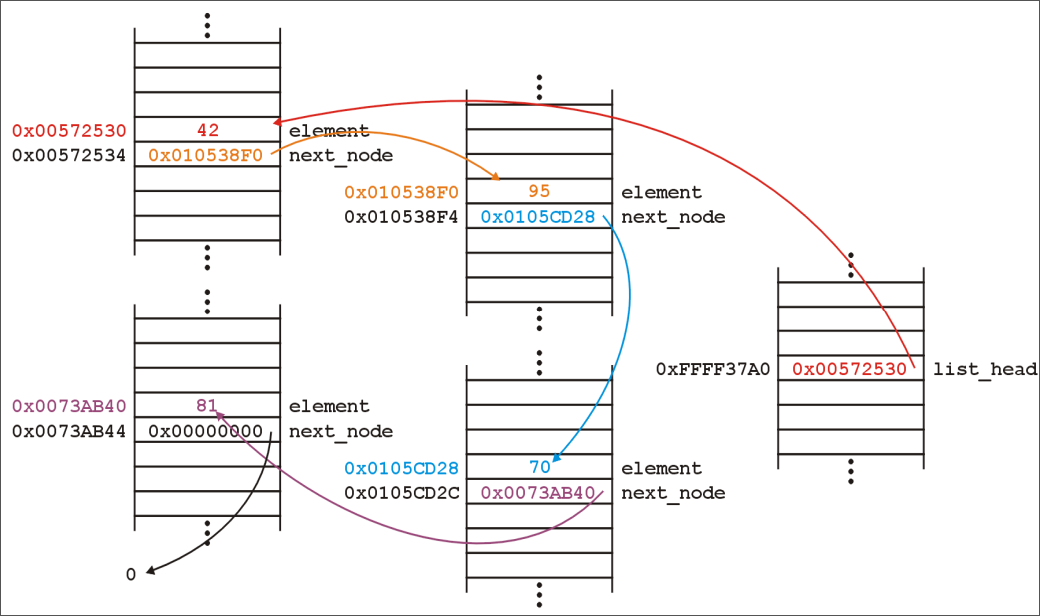
\includegraphics[width=0.35\textwidth]{ExempleListeChaine.png}
    \end{center}
  \end{figure}


  \begin{Definitionx}{Liste S. chaînée}{}
    Une \textbf{liste simplement chaînée} est une structure 
    de données concrète 
    constituée d'une \textit{séquence de nœuds} à partir
    d'une référence vers 
    le \textbf{noeud de tête}, où chaque nœud 
    contient deux références : 
    vers un \texttt{\textbf{E}}   et vers le \textbf{nœud suivant}. 
    On gardera aussi une référence sur le dernier 
    nœud et un entier 
    pour le nombre d’éléments dans la liste.     
  \end{Definitionx}

  \begin{figure}[H]
    \begin{center}
      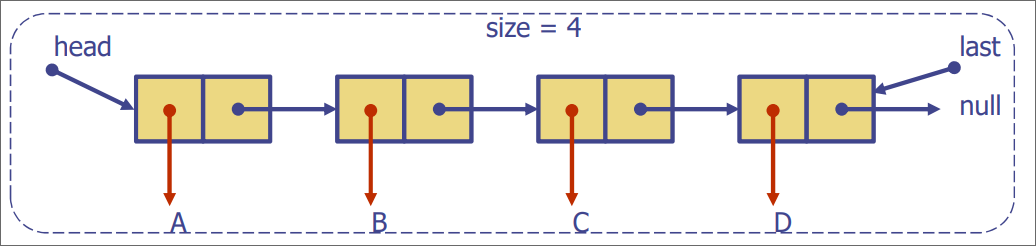
\includegraphics[width=0.33\textwidth]{ListeSChainee.png}
    \end{center}
  \end{figure}



  \begin{lstlisting}
   initialisation(varElement, varNext)
   element <-- varElement // Assigne E
   next <-- varNext  // specifie prochain noeud


   Class LinkList(List) 
   initialisation()
   head <-- null 
   next <-- null 
   size <-- 0

   fonction len() 
      retourner size 

  fonction str() 
    Si isEmpty() 
      retourner "[] (size = 0)"
    Si non : 
    PP <- "["
    curr <- head 
    tant que curr != null faire 
      // (concat)
      PP <- PP + curr.next + " " 
      curr <- curr.next

    Fin tant que 

    PP <- PP + "]" 
    PP <- PP + "(size = " + size +")"

  fonction isEmpty() 
      retourner size = 0
  \end{lstlisting}

  \section{Liste doublement chaînée}
  \begin{Definitionx}{Liste D. chaînée}{}
    Une \textbf{liste doublement chaînée} est une structure de 
    données constituée d'une \textit{séquence de nœuds} à partir 
    de références vers les nœuds de tête et de queue, 
    où chaque nœud contient \textbf{trois références} : 
    vers un \texttt{\textbf{E}}  , 
    vers le \textbf{nœud suivant} et vers le \textbf{nœud précédent}.
    On gardera aussi un entier pour le nombre d’éléments 
    dans la liste.     
  \end{Definitionx}

  \begin{lstlisting}
Class DoublyLinkedNode() 

// Methode generale d'initialisation
initialisation(varE, varPrev, varNext) 
  element <-- varE 
  prev <-- varPrev 
  next <-- varNext 


// initialisation pour 
// engendrer la fonction str()


initialisation()
  head <-- DoublyLinkedNote(null, null, null)
  tail <-- DoublyLinkedNode(null, null, null) 
  head.next <-- tail
  tail.prev <-- head 
  size <-- 0 

fonction len() 
  retourner size 

fonction str() 
  Si isEmpty() 
    retourner 
    "[] (size = 0)"
  Sinon :
    PP <-- "[" 
    curr <-- head.next

    tant que curr.next != tail faire :
      PP <-- PP + curr.element + "" 
      curr <-- curr.next 
    Fin tant que 

    PP <-- PP + "]" + 
    "size = (" + size + ")"
  Fin si 

fonction isEmpty() 
  retourner size = 0

  \end{lstlisting}

  \chapter{Liste généralisée}
  \begin{Definitionx}{Liste G.}{}
      Liste dans laquelle les éléments 
      peuvent être des sous-listes 
      Si un \texttt{E} de la liste 
      \textbf{n'est pas} une sous-liste, il est dit 
      \textcolor{red}{atomique}. Les liste 
      généralisées peuvent être représentées 
      par des représentations 
      séquentielles ou chaînées. 
  \end{Definitionx}

  \paragraph{Liste généralisée 1}
  \begin{lstlisting}
(a_1, a_2, 
  (b_1, 
    (c_1, c_2), 
  b_3), 
a_4, 
  (d_1, d_2) 
a_6) 
  \end{lstlisting}

  \begin{note}{}{}
      On utilise \textbf{0} pour représenter un 
      atome et \textbf{1} pour représenter une 
      sous-liste (Parfois T/F)
  \end{note}

  \paragraph{Liste généralisée 2}
  \begin{figure}[H]
    \begin{center}
      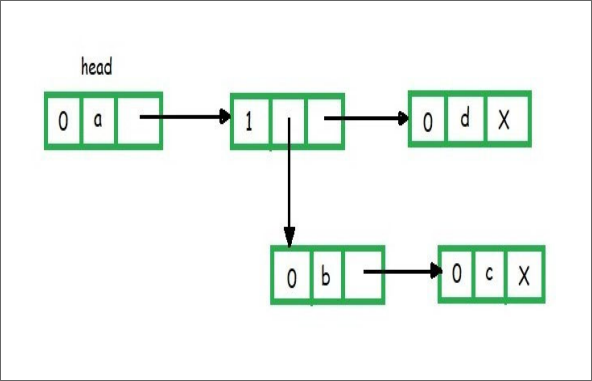
\includegraphics[width=0.33\textwidth]{ListeGen2.png}
    \end{center}
  \end{figure}

  \paragraph{Liste généralisée 3}

  \begin{figure}[H]
    \begin{center}
      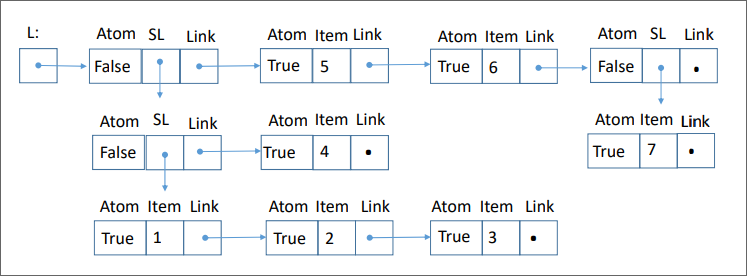
\includegraphics[width=0.33\textwidth]{Listegen.png}
    \end{center}
  \end{figure}


  \chapter{File}
  Pour l'implémentation, on utilise un tableau circulaire de 
  \textcolor{red}{taille $N$}, ainsi que 
  \textit{deux variables} qui gardent trace de 
  l'\textbf{avant} et l'\textbf{arrière} : 
  \textcolor{red}{$f$} et \textcolor{red}{$r$}.       
  \begin{itemize}
    \item [$\rhd$ ] \textcolor{red}{$f$} 
      index directement sur la valeur  
    \item [$\rhd$ ] \textcolor{red}{$r$} 
      index 1ere case vide après valeur. 
  \end{itemize}


  \begin{figure}[H]
    \begin{center}
      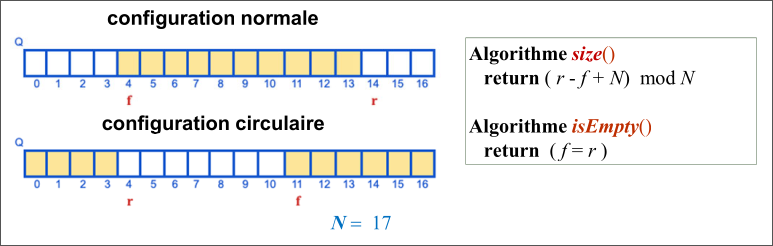
\includegraphics[width=0.33\textwidth]{FileSurTableau.png}
    \end{center}
  \end{figure}

  \begin{lstlisting}
// Algorithme size() 
retourne (r - f + N) mod N 

// Algorithme isEmpty() 
retourn (f = r)


// Algorithme Enqueue(x) 
Si size() = N - 1 faire : 
  retourne Erreur 
Sinon : 
  Q[r] <-- x 
  r <-- (r+1) mod N


// Algorithme Dequeue()
Si Q iseEmpty() faire : 
  retourne erreur 
Sinon :
  x <-- Q[f] 
  f <-- (f + 1) mod N 
  retourne x
  \end{lstlisting}


  \paragraph{Variante}
  \begin{itemize}
    \item [$\rhd$ ] \textcolor{red}{$f$} 
      index directement sur la valeur  
    \item [$\rhd$ ] \textcolor{red}{$r$} 
      
      index \textcolor{red}{directement sur case fin}. 
  \end{itemize}

\begin{lstlisting}
 // Algorithme size() 
retourne ((r - f + N) mod N) + 1

// Algorithme isEmpty() 
retourne (f = (r + 1) mod N)

// Algorithme Enqueue(x) 
Si ((r + 1) mod N) = f alors 
  retourne Erreur // La file est pleine
Sinon : 
  Q[r] <-- x 
  r <-- (r + 1) mod N

// Algorithme Dequeue()
Si isEmpty() alors 
  retourne erreur 
Sinon :
  x <-- Q[f] 
  f <-- (f + 1) mod N 
  retourne x
\end{lstlisting}
  
  
  
  
  






    














    \end{multicols*}


\end{document}

